%%%%%%%%%%%%%%%%%%%%%%%%%%%%%%%%%%%%%%%%%%%%%%%%%%%%%%%%%%%%%%%%%%%%%%%%
% Escuela Politécnica Superior de la Universidad de Alicante
% Realizado por: Jose Manuel Requena Plens
% Contacto: info@jmrplens.com / Telegram:@jmrplens
%%%%%%%%%%%%%%%%%%%%%%%%%%%%%%%%%%%%%%%%%%%%%%%%%%%%%%%%%%%%%%%%%%%%%%%%


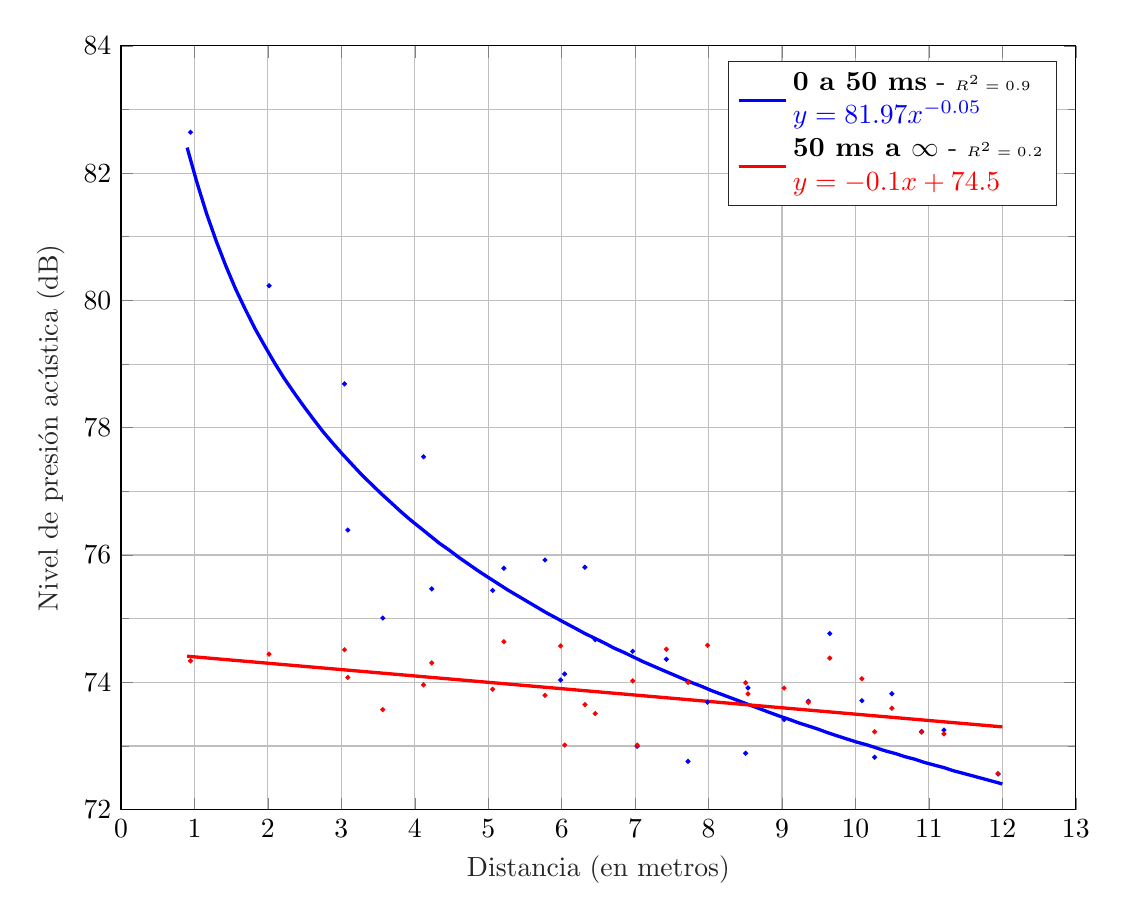
\begin{tikzpicture}

\begin{axis}[%
width=\textwidth,
height=0.8\textwidth,
at={(0\textwidth,0\textwidth)},
scale only axis,
xmin=0,
xmax=13,
xlabel style={font=\color{white!15!black}},
xlabel={Distancia (en metros)},
ymin=72,
ymax=84,
xmajorgrids,
xminorgrids,
ymajorgrids,
yminorgrids,
minor y tick num= 1,
ylabel style={font=\color{white!15!black}},
ylabel={Nivel de presión acústica (dB)},
axis background/.style={fill=white},
legend style={legend cell align=left, align=left, draw=white!15!black}
]
\addplot [color=blue, only marks,mark size=0.7pt, forget plot]
  table[row sep=crcr]{%
0.945832966226064	82.6420079958914\\
2.0155892438689	80.2303554003687\\
3.04292622322659	78.6881045727944\\
3.08781476128345	76.3922767253641\\
3.56407070636934	75.0100820613083\\
4.11885906532379	77.543416910588\\
4.23076825174815	75.4693527412033\\
5.0601383380299	75.444066602597\\
5.21338661524349	75.7915413606487\\
5.7725297747175	75.9216852693002\\
5.98493107729738	74.0366131016921\\
6.04070360140274	74.1312005354213\\
6.31685048105462	75.8077293987195\\
6.45653932071973	74.6715272292603\\
6.96725196903341	74.4875231200194\\
7.02797979507625	72.99559772715\\
7.42526767194288	74.3627070297666\\
7.72055049850721	72.7576960941599\\
7.98590007450632	73.6889279610953\\
8.5047104595042	72.8855286933151\\
8.53670896774629	73.9130300559927\\
9.02858792946051	73.4166836406291\\
9.35746226281464	73.702884884372\\
9.65012953280939	74.7664519770778\\
10.0878639959111	73.71153847285\\
10.2617201287114	72.822938510167\\
10.4960706933595	73.8196487744781\\
10.8998853204976	73.227376539976\\
11.2050211958747	73.2501558174068\\
11.9413148354777	72.5594130132974\\
};
\addplot[color=blue,domain=0.9:12, samples=85,line width=1.2]{81.97*x^(-0.05)};
\addlegendentry{\textbf{0 a 50 ms} - \tiny{$R^2 = 0.9$}\\$\color{blue}y = 81.97·x^{-0.05}$}

\addplot [color=red, only marks,mark size=0.7pt, forget plot]
  table[row sep=crcr]{%
0.945832966226064	74.3367942916818\\
2.0155892438689	74.4428555138378\\
3.04292622322659	74.511850056859\\
3.08781476128345	74.0768454974658\\
3.56407070636934	73.570968193684\\
4.11885906532379	73.960193320587\\
4.23076825174815	74.3058561007808\\
5.0601383380299	73.8906487606386\\
5.21338661524349	74.638243792516\\
5.7725297747175	73.793741140568\\
5.98493107729738	74.5716721982254\\
6.04070360140274	73.0144941684959\\
6.31685048105462	73.6493891472023\\
6.45653932071973	73.509586766673\\
6.96725196903341	74.0237029187056\\
7.02797979507625	73.0128244006444\\
7.42526767194288	74.5199342918284\\
7.72055049850721	73.9989506580923\\
7.98590007450632	74.5821265722156\\
8.5047104595042	73.9925438985215\\
8.53670896774629	73.8193785231492\\
9.02858792946051	73.9085522734068\\
9.35746226281464	73.6859259436621\\
9.65012953280939	74.3803174126395\\
10.0878639959111	74.0555050161735\\
10.2617201287114	73.2230389538318\\
10.4960706933595	73.5932649217609\\
10.8998853204976	73.2166557384589\\
11.2050211958747	73.1901137726248\\
11.9413148354777	72.5672282318972\\
};
\addplot[color=red,domain=0.9:12, samples=85,line width=1.2]{-0.1*x+74.5};
\addlegendentry{\textbf{50 ms a $\infty$} - \tiny{$R^2 = 0.2$}\\$\color{red}y = -0.1·x+74.5$}

\end{axis}
\end{tikzpicture}%